\documentclass[border=6pt,tikz]{standalone}
\usepackage{amsmath,amssymb}
\usepackage{tikz}
\usetikzlibrary{arrows.meta,calc,decorations.pathreplacing,patterns,shapes.geometric,positioning,shadings}

\begin{document}
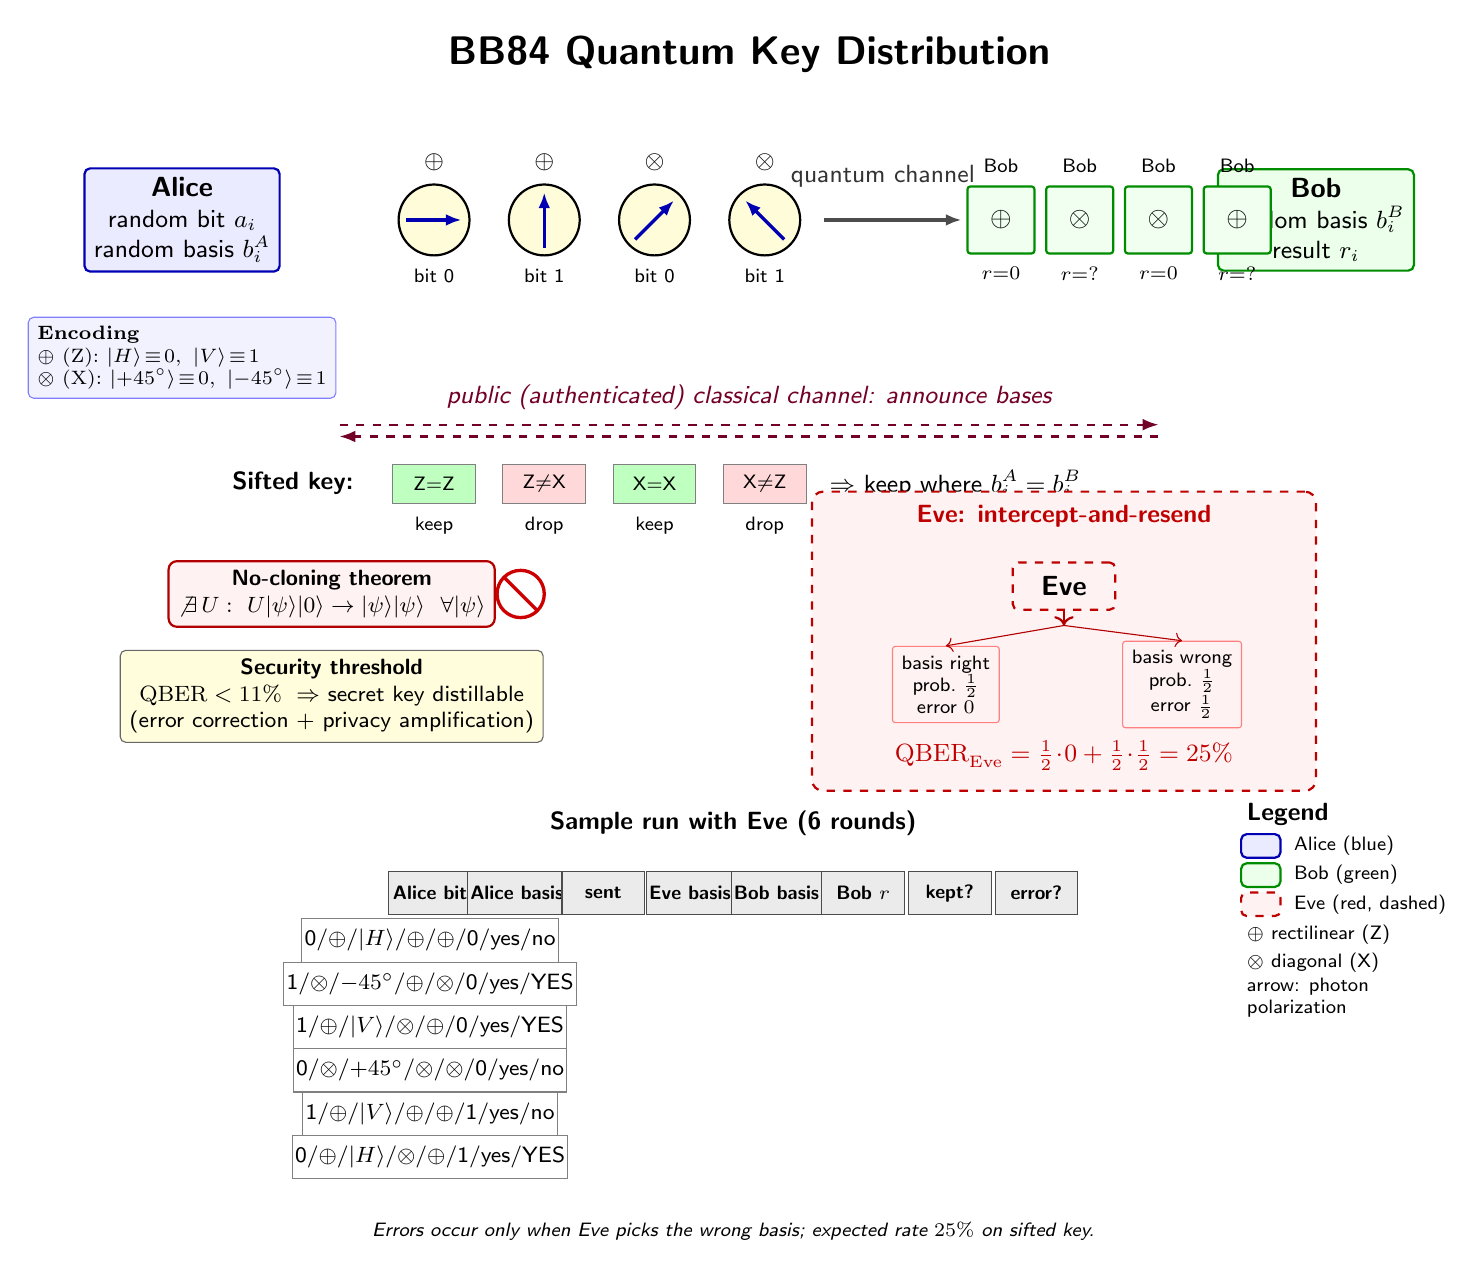
\begin{tikzpicture}[
  font=\sffamily,
  alice/.style={draw=blue!70!black, thick, fill=blue!8, rounded corners=2pt, align=center},
  bob/.style={draw=green!55!black, thick, fill=green!8, rounded corners=2pt, align=center},
  eve/.style={draw=red!75!black, thick, dashed, fill=red!5, rounded corners=2pt, align=center},
  photon/.style={draw=black, thick, fill=yellow!15, circle, minimum size=9mm, inner sep=0pt},
  basislabel/.style={font=\sffamily\small},
  chan/.style={-{Latex[length=2mm]}, very thick, gray!60!black},
  pubchan/.style={-{Latex[length=2mm]}, thick, dashed, purple!60!black},
  cell/.style={draw=black!50, minimum width=1.05cm, minimum height=0.55cm, inner sep=1pt, font=\footnotesize\sffamily},
  hdr/.style={draw=black!70, fill=black!8, minimum width=1.05cm, minimum height=0.55cm, inner sep=1pt, font=\scriptsize\sffamily\bfseries}
]

% ===================== TITLE =====================
\node[font=\Large\sffamily\bfseries] at (0,5.9) {BB84 Quantum Key Distribution};

% ===================== ALICE =====================
\node[alice, minimum width=2.4cm, minimum height=1.1cm] (alice) at (-7.2, 3.8) {\bfseries Alice\\[-1pt] \small random bit $a_i$\\[-1pt] \small random basis $b^A_i$};

% Four example photons from Alice (encoded polarizations)
\def\photY{3.8}
\foreach \i/\x/\ang/\basis/\bit in {1/-4.0/0/$\oplus$/0, 2/-2.6/90/$\oplus$/1, 3/-1.2/45/$\otimes$/0, 4/0.2/135/$\otimes$/1} {
  \node[photon] (pA\i) at (\x,\photY) {};
  \draw[-{Latex[length=2mm]}, very thick, blue!70!black] ($(pA\i.center)+(\ang+180:3.5mm)$) -- ($(pA\i.center)+(\ang:3.5mm)$);
  \node[basislabel, above=1pt of pA\i] {\basis};
  \node[basislabel, below=1pt of pA\i] {\scriptsize bit \bit};
}

% Encoding legend
\node[draw=blue!50, fill=blue!5, rounded corners=2pt, align=left, font=\scriptsize] (enc) at (-7.2, 2.05) {
\textbf{Encoding}\\
$\oplus$ (Z): $|H\rangle\!\equiv\!0,\ |V\rangle\!\equiv\!1$\\
$\otimes$ (X): $|{+}45^{\circ}\rangle\!\equiv\!0,\ |{-}45^{\circ}\rangle\!\equiv\!1$
};

% ===================== QUANTUM CHANNEL =====================
\node[font=\small\sffamily, gray!40!black] at (1.7, \photY+0.55) {quantum channel};
\draw[chan] (0.95, \photY) -- (2.7, \photY);

% ===================== BOB =====================
\node[bob, minimum width=2.4cm, minimum height=1.1cm] (bob) at (7.2, 3.8) {\bfseries Bob\\[-1pt] \small random basis $b^B_i$\\[-1pt] \small result $r_i$};

% Bob basis choice (squares)
\def\photYb{3.8}
\foreach \i/\x/\basis/\result in {1/3.2/$\oplus$/0, 2/4.2/$\otimes$/?, 3/5.2/$\otimes$/0, 4/6.2/$\oplus$/?} {
  \node[draw=green!55!black, thick, fill=green!6, minimum width=0.85cm, minimum height=0.85cm, rounded corners=1pt] (pB\i) at (\x,\photYb) {\basis};
  \node[basislabel, above=1pt of pB\i] {\scriptsize Bob};
  \node[basislabel, below=1pt of pB\i] {\scriptsize $r{=}\result$};
}

% ===================== PUBLIC CHANNEL =====================
\node[font=\small\sffamily\itshape, purple!60!black] at (0, 1.55) {public (authenticated) classical channel: announce bases};
\draw[pubchan] (-5.2, 1.2) -- (5.2, 1.2);
\draw[pubchan] (5.2, 1.05) -- (-5.2, 1.05);

% Sifted key row
\node[font=\small\sffamily\bfseries, anchor=east] at (-4.9, 0.45) {Sifted key:};
\foreach \i/\x/\match/\sift/\clr in {1/-4.0/{Z=Z}/keep/green!25, 2/-2.6/{Z$\ne$X}/drop/red!15, 3/-1.2/{X=X}/keep/green!25, 4/0.2/{X$\ne$Z}/drop/red!15} {
  \node[draw=black!50, fill=\clr, minimum width=1.05cm, minimum height=0.5cm, font=\scriptsize\sffamily] at (\x, 0.45) {\match};
  \node[font=\scriptsize\sffamily, anchor=north] at (\x, 0.15) {\sift};
}
\node[font=\small\sffamily, anchor=west] at (0.9, 0.45) {$\Rightarrow$ keep where $b^A_i = b^B_i$};

% ===================== NO-CLONING THEOREM =====================
\node[draw=red!70!black, thick, fill=red!5, rounded corners=3pt, align=center, font=\footnotesize\sffamily] (nc) at (-5.3, -0.95) {
\textbf{No-cloning theorem}\\
$\not\exists\, U:\ U|\psi\rangle|0\rangle \to |\psi\rangle|\psi\rangle\ \ \forall |\psi\rangle$
};
% Red prohibit symbol
\begin{scope}[shift={(-2.9,-0.95)}]
  \draw[red!80!black, very thick] (0,0) circle (0.3);
  \draw[red!80!black, very thick] (-0.212,0.212) -- (0.212,-0.212);
\end{scope}

% Security threshold box
\node[draw=black!60, fill=yellow!14, rounded corners=2pt, align=center, font=\footnotesize\sffamily] at (-5.3, -2.25) {
\textbf{Security threshold}\\
$\mathrm{QBER}<11\%\ \Rightarrow$ secret key distillable\\
(error correction + privacy amplification)
};

% ===================== EVE PANEL =====================
\node[eve, minimum width=6.4cm, minimum height=3.8cm, rounded corners=4pt] (evepanel) at (4.0, -1.55) {};
\node[font=\small\sffamily\bfseries, red!75!black, anchor=north] at ($(evepanel.north)+(0,-0.06)$) {Eve: intercept-and-resend};

\node[eve, minimum width=1.3cm, minimum height=0.6cm] (eveBox) at (4.0, -0.85) {\textbf{Eve}};

% Branch tree
\coordinate (evebr) at (4.0,-1.35);
\draw[red!70!black, ->, thick] (eveBox.south) -- (evebr);

\node[font=\scriptsize\sffamily, align=center, draw=red!50, fill=red!5, rounded corners=1pt] (correct) at (2.5, -2.1) {basis right\\ prob.\ $\tfrac12$\\ error $0$};
\node[font=\scriptsize\sffamily, align=center, draw=red!50, fill=red!5, rounded corners=1pt] (wrong) at (5.5, -2.1) {basis wrong\\ prob.\ $\tfrac12$\\ error $\tfrac12$};

\draw[red!70!black, ->] (evebr) -- (correct.north);
\draw[red!70!black, ->] (evebr) -- (wrong.north);

\node[font=\small\sffamily\bfseries, red!75!black, align=center] at (4.0, -3.0) {$\mathrm{QBER}_{\mathrm{Eve}}=\tfrac12\!\cdot\!0+\tfrac12\!\cdot\!\tfrac12=25\%$};

% ===================== SAMPLE RUN TABLE =====================
\begin{scope}[shift={(-0.2, -5.9)}]
  \node[font=\small\sffamily\bfseries, anchor=south] at (0, 1.75) {Sample run with Eve (6 rounds)};
  % Header
  \foreach \c/\lbl in {0/{Alice bit}, 1/{Alice basis}, 2/{sent}, 3/{Eve basis}, 4/{Bob basis}, 5/{Bob $r$}, 6/{kept?}, 7/{error?}} {
    \node[hdr] at (\c*1.1 - 3.85, 1.15) {\lbl};
  }

  % Rows
  \def\rowA{0/$\oplus$/$|H\rangle$/$\oplus$/$\oplus$/0/yes/no}
  \def\rowB{1/$\otimes$/${-}45^{\circ}$/$\oplus$/$\otimes$/0/yes/YES}
  \def\rowC{1/$\oplus$/$|V\rangle$/$\otimes$/$\oplus$/0/yes/YES}
  \def\rowD{0/$\otimes$/${+}45^{\circ}$/$\otimes$/$\otimes$/0/yes/no}
  \def\rowE{1/$\oplus$/$|V\rangle$/$\oplus$/$\oplus$/1/yes/no}
  \def\rowF{0/$\oplus$/$|H\rangle$/$\otimes$/$\oplus$/1/yes/YES}

  \foreach \row [count=\ri from 0] in {\rowA, \rowB, \rowC, \rowD, \rowE, \rowF} {
    \foreach \v [count=\ci from 0] in \row {
      \pgfmathsetmacro\yy{0.55 - \ri*0.55}
      \pgfmathsetmacro\xx{\ci*1.1 - 3.85}
      \ifnum\ci=7
        \ifnum\ri=1 \node[cell, fill=red!22] at (\xx, \yy) {\v};
        \else\ifnum\ri=2 \node[cell, fill=red!22] at (\xx, \yy) {\v};
        \else\ifnum\ri=5 \node[cell, fill=red!22] at (\xx, \yy) {\v};
        \else \node[cell] at (\xx, \yy) {\v};
        \fi\fi\fi
      \else
        \node[cell] at (\xx, \yy) {\v};
      \fi
    }
  }

  \node[font=\scriptsize\sffamily\itshape, anchor=north] at (0, -2.9) {Errors occur only when Eve picks the wrong basis; expected rate $25\%$ on sifted key.};
\end{scope}

% ===================== LEGEND =====================
\begin{scope}[shift={(6.2, -5.3)}]
  \node[font=\small\sffamily\bfseries, anchor=west] at (0,1.55) {Legend};
  \node[alice, minimum width=0.5cm, minimum height=0.3cm] at (0.3, 1.15) {};
  \node[anchor=west, font=\scriptsize\sffamily] at (0.6, 1.15) {Alice (blue)};
  \node[bob, minimum width=0.5cm, minimum height=0.3cm] at (0.3, 0.78) {};
  \node[anchor=west, font=\scriptsize\sffamily] at (0.6, 0.78) {Bob (green)};
  \node[eve, minimum width=0.5cm, minimum height=0.3cm] at (0.3, 0.41) {};
  \node[anchor=west, font=\scriptsize\sffamily] at (0.6, 0.41) {Eve (red, dashed)};
  \node[font=\scriptsize\sffamily, anchor=west] at (0.0, 0.02) {$\oplus$ rectilinear (Z)};
  \node[font=\scriptsize\sffamily, anchor=west] at (0.0, -0.33) {$\otimes$ diagonal (X)};
  \node[font=\scriptsize\sffamily, anchor=west, align=left] at (0.0, -0.78) {arrow: photon\\ polarization};
\end{scope}

\end{tikzpicture}
\end{document}
